\documentclass[compress]{beamer}
\usepackage{hyperref}
\usepackage[T1]{fontenc}
\usepackage{beramono}
\usepackage{xcolor}
\usepackage[ruled]{algorithm2e}
\usepackage{tikz}
\usetheme{Warsaw}
\usecolortheme{crane}

\def\HiLi{\leavevmode\rlap{\hbox to \hsize{\color{yellow!50}\leaders\hrule height .8\baselineskip depth .5ex\hfill}}}
\usefonttheme[onlymath]{serif}

\newenvironment{definitionblock}[1]{
  \setbeamercolor{block title}{bg=cyan}
  \begin{block}{#1}}{\end{block}
}

\author{Wing}
\title{Suffix Tree (Ukkonen's algorithm)}  

\begin{document}
\date{\today} 

\frame[plain]{\titlepage} % [plain] means it doesn't show the section above the Header 

\frame[plain]{\frametitle{Table of contents}
\small
\tableofcontents[hideallsubsections]
}  

\section{Suffix Trie}
\begin{frame}[fragile,plain] \frametitle{Trie}
\begin{block}{Trie}
    An ordered tree data structure used to store a dynamic set or map where the keys are usually strings
\end{block}
\end{frame}

\begin{frame}[fragile,plain] \frametitle{Suffix Trie}
    \begin{figure}
        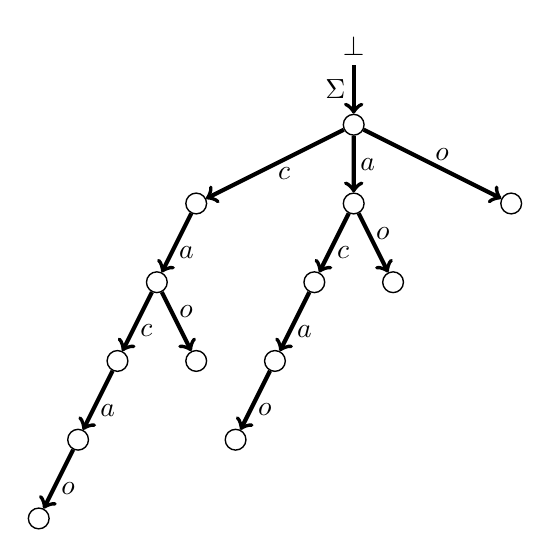
\begin{tikzpicture}[level distance=10mm,->,line width=1.5pt]
            \tikzstyle{every node}=[draw,circle,inner sep=1pt,minimum size=7.5pt,line width=0.5pt]
            \tikzstyle{sll}=[bend left,dashed,line width=0.5pt,->]
            \tikzstyle{slr}=[bend right,dashed,line width=0.5pt,->]
            \tikzstyle{level 1}=[sibling distance=10mm]
            \tikzstyle{level 2}=[sibling distance=20mm]
            \tikzstyle{level 3}=[sibling distance=10mm]
            \node [draw=none] (bottom) {$\bot$}
                child {node (root) {}
                    child {node {}
                        child{node {}
                            child{node {}
                                child{node {}
                                    child{node {}
                                        edge from parent
                                        node[auto,draw=none] {$o$}
                                    }
                                    child{node[draw=none] {}
                                        edge from parent[draw=none]
                                        node[auto,draw=none] {}
                                    }
                                    edge from parent
                                    node[auto,draw=none] {$a$}
                                }
                                child{node[draw=none] {}
                                    edge from parent[draw=none]
                                    node[auto,draw=none] {}
                                }
                                edge from parent
                                node[auto,draw=none] {$c$}
                            }
                            child{node {}
                                edge from parent
                                node[auto,draw=none] {$o$}
                            }
                            edge from parent
                            node[auto,draw=none] {$a$}
                        }
                        child{node[draw=none] {}
                            edge from parent[draw=none]
                            node[auto,draw=none] {}
                        }
                        edge from parent
                        node[auto,draw=none] {$c$}
                    }
                    child {node {}
                        child{node {}
                            child{node {}
                                child{node {}
                                    edge from parent
                                    node[auto,draw=none] {$o$}
                                }
                                child{node[draw=none] {}
                                    edge from parent[draw=none]
                                    node[auto,draw=none] {}
                                }
                                edge from parent
                                node[auto,draw=none] {$a$}
                            }
                            child{node[draw=none] {}
                                edge from parent[draw=none]
                                node[auto,draw=none] {}
                            }
                            edge from parent
                            node[auto,draw=none] {$c$}
                        }
                        child{node {}
                            edge from parent
                            node[auto,draw=none] {$o$}
                        }
                        edge from parent
                        node[auto,draw=none] {$a$}
                    }
                    child {node {}
                        edge from parent
                        node[auto,draw=none] {$o$}
                    }
                    edge from parent
                    node[draw=none,left] {$\Sigma$}
                }
                ;
                % \draw[style=slr] (root) to (bottom);
            \end{tikzpicture}
            \caption{Suffix Trie for $``cacao"$} \label{fig:M1}
    \end{figure}
\end{frame}

\begin{frame}[fragile,plain] \frametitle{Suffix Trie}
    \begin{itemize}
    \item Proposed by Esko Ukkonen (University of Helsinki, Finland)
    \item An algorithm easier to grasp than the those in the literature at that time
    \item On-line algorithm: Processes the string symbol by symbol from left to right, and always has the suffix tree for the scanned
part of the string ready
    \end{itemize}
\end{frame}

\begin{frame}[fragile,plain] \frametitle{Construction of Suffix Trie}
    \begin{definitionblock}{String}
        Let $T = t_1t_2\cdots t_n$ be a string over alphabet $\Sigma$
    \end{definitionblock}
    \begin{definitionblock}{Substring}
        Each string $x$ s.t. $T = uxv$ for some (possibly empty) string $u$ and $v$ is a \underline{substring} of $T$
    \end{definitionblock}
    \begin{definitionblock}{Suffix}
        $T_i = t_i\cdots t_n $ where $ 1 \leq i \leq n + 1 $
        \begin{itemize}
            \item $T_{n+1} = \epsilon$ is the \emph{empty} suffix
        \end{itemize}
    \end{definitionblock}
\end{frame}

\begin{frame}[fragile,plain] \frametitle{Construction of Suffix Trie}
    \begin{definitionblock}{Set of all suffixes of $T$}
        $\sigma(T)$
    \end{definitionblock}
    The suffix trie of $T$ is a trie representing $\sigma(T)$
\end{frame}

\begin{frame}[fragile,plain] \frametitle{Construction of Suffix Trie}
    \begin{definitionblock}{Suffix Trie}
    Denote suffix trie of $T$ as $STrie(T) = (Q \cup \lbrace\bot\rbrace, root, F, g, f)$
    \hfill \break
    \hfill \break
    Define such a trie as an augmented deterministic finite-state automaton which has a tree-shaped transition graph representing the trie for $\sigma(T)$
    \hfill \break
    \hfill \break
    augmented with
    \begin{itemize}
        \item $f$ : \underline{suffix function}
        \item $\bot$ : \underline{auxiliary state}
    \end{itemize}
    \end{definitionblock}
\end{frame}

\begin{frame}[fragile,plain] \frametitle{Construction of Suffix Trie}
    \begin{definitionblock}{Set $Q$ of the states of $STrie(T)$}
    The set $Q$ of the states of $STrie(T)$ can be put in a one-to-one correspondence with the substrings of $T$.
    \hfill \break
    \hfill \break
    Denote $\bar{x}$ the state that corresponds to a substring $x$
    \hfill \break
    Shorthand: $\bar{x} \sim x$
    \begin{itemize}
        \item $root \sim \epsilon$
        \item   $\sigma(T) \sim $ set $F$ of final states
    \end{itemize}

    \end{definitionblock}
\end{frame}

\begin{frame}[fragile,plain] \frametitle{Construction of Suffix Trie}
    \begin{definitionblock}{Transition function $g$}
        $
        \begin{cases}
            g(\bar{x}, a) = \bar{y} \  & \forall \bar{x}, \bar{y} \in Q \ \mbox{s.t.} \ y = xa, \ \mbox{where} \ a \in \Sigma
        \\
            g(\bot, a) = root \ & \forall a \in \Sigma
        \end{cases}
        $
    \end{definitionblock}
    \begin{definitionblock}{Suffix function $f$}
        $\forall \bar{x} \in Q,$ \\
        $\begin{cases} f(\bar{x}) = \bar{y} & \mbox{if} \ \bar{x} \neq root, \mbox{then}\ x = ay, a \in \Sigma \\ f(root) = \bot \\
            f(\bot) \ \mbox{is undefined}
        \end{cases}$
    \end{definitionblock}
    $\bot \sim a^{-1} \ \forall a \in \Sigma$
    \hfill \break
    $a^{-1}a=\epsilon$
\end{frame}

\begin{frame}[fragile,plain] \frametitle{Construction of Suffix Trie}
    \begin{definitionblock}{Suffix Link}
        $f(r)$ is the suffix link of state $r$
    \end{definitionblock}

    \begin{definitionblock}{Prefix}
        $T^{i} = t_1\cdots t_i$ of $T$ for $0 \leq i \leq n $
    \end{definitionblock}
\end{frame}

\begin{frame}[fragile,plain] \frametitle{Construction of Suffix Trie}
    \begin{block}{Key observation}
        How is $STrie(T^i)$ obtained from $STrie(T^{i-1})$?
        \hfill \break
        \hfill \break
        The suffixes of $T^i$ can be obtained by catenating $t_i$ to the end of each suffix of $T^{i-1}$ and by adding an empty suffix, i.e.
        $$\sigma(T^i) = \sigma(T^{i-1})t_i \cup \{ \epsilon \} $$
    \end{block}
        $STrie(T^{i-1})$ accepts $\sigma(T^{i-1})$, to make it accept $\sigma(T^{i})$,
        examine $F_{i-1}$ of $STrie(T^{i-1})$
        \begin{itemize}
            \item $r \in F_{i-1}$ doesn't have a $t_i$-transition $\Rightarrow$ add transition $r \rightarrow$ new state
            \item $r \in F_{i-1}$ has a $t_i$-transition $\Rightarrow$ follow the transition to the old state
            \item All such states plus $root$ will be $F_i$ of $STrie(T^i)$
        \end{itemize}
\end{frame}

\begin{frame}[fragile,plain] \frametitle{Construction of Suffix Trie}
    How to find states $r \in F_{i-1}$ that get new transitions?
    \hfill \break
    \hfill \break
    From definition of the suffix function $f$,
    \hfill \break
    $r \in F_{i-1} \Leftrightarrow r = f^j (\overline{t_1\cdots t_{i-1}})$ for some $ 0 \leq j \leq i - 1$
    \begin{definitionblock}{Boundary path}
        Boundary path of $STrie(T^{i-1})$: \\
        Path starting from deepest state $\overline{t_1\cdots t_{i-1}}$ of $STrie(T^{i-1})$, following the suffix links and ending at $\bot$
    \end{definitionblock}
    $\therefore $ All states in $F_{i-1}$ are on the \underline{boundary path} of $STrie(T^{i-1})$
\end{frame}

\begin{frame}[fragile,plain] \frametitle{Construction of Suffix Trie}
    The boundary path is traversed. \\
	\hfill \break
    If a state $\bar{z}$ on the boundary path does not have a transition on $t_i$ yet,
    add a new state $\overline{zt_i}$ and a new transition $g(\bar{z}, t_i) = \overline{zt_i}$ \\
	\hfill \break
	To update $f$, new states $\overline{zt_i}$ are linked together with new suffix links starting from $\overline{t_1\cdots t_{i}}$. \\
	Obviously, this is the boundary path of $STrie(T^i)$
\end{frame}

\begin{frame}[fragile,plain] \frametitle{Construction of Suffix Trie}
    \begin{block}{Observation}
        The traversal over $F_{i-1}$ along the boundary path can be stopped immediately when the first state $\bar{z}$ is found s.t. state $\overline{zt_i}$ (and hence also transition $g(\bar{z}, t_i) = \overline{zt_i}$) already exists.
    \end{block}
    Let namely $\overline{zt_i}$ already be a state. \\
    \hfill \break
    Then $STrie(T^{i-1})$ has to contain state $\overline{z't_i}$ and transition $g(z', t_i) = \overline{z't_i} \ \forall z' = f^j(\bar{z}), j \leq 1$. \\
    In other words, if $\overline{zt_i}$ is a substring of $T_{i-1}$ then every suffix of $\overline{zt_i}$ is a substring of $T_{i-1}$.\\
    \hfill \break
    Such $\bar{z}$ must exist as $\bot$ is the last state on the boundary path that has the $t_i$-transition $\forall t_i$
\end{frame}

\frame[plain]{\frametitle{test}
    $$\sum_{n=1}^{\infty} 2^{-n} = 1$$ \\
    $$\mathcal{O}(n)$$
	\begin{block}{block name}
        block
	\end{block}
    \pause
	\begin{exampleblock}{exampleblock name}
        exampleblock
	\end{exampleblock}
	\begin{alertblock}{alertblock name}
        alertblock
	\end{alertblock}
}

\begin{frame}[fragile,plain]\frametitle{High level thinking}
    \LinesNumbered
    \begin{procedure}[H]
     \caption{Evolutionary procedure(x)}
     initialize population \;
     \HiLi\For( \emph{Evolutionary loop}){$g := 1$ to $G_{max}$}
     {
        \HiLi do things \;
        evolve population \;
     }
     celebrate \;
     \end{procedure}
\end{frame}

\section{Suffix Tree}
\begin{frame}[fragile,plain]
    hi
\end{frame}

\section{Usage of Suffix Tree}
\begin{frame}[fragile,plain]
    hi
\end{frame}

% \section{References}
% \begin{frame}[fragile,plain]\frametitle{References}
%     Original Paper: \\
%     \url{https://www.cs.helsinki.fi/u/ukkonen/SuffixT1withFigs.pdf} \\
%     \hfill \break
%     Wikipedia for the definition of Trie
% \end{frame}

\end{document}
